\documentclass{beamer}

\usetheme{Warsaw}

\setbeamertemplate{itemize items}[circle]


\usepackage[slovene]{babel}
\usepackage[utf8]{inputenc}
\usepackage[T1]{fontenc}
\usepackage{lmodern}

\usepackage{amsfonts, amsmath, amsthm}
\usepackage{enumitem}
\usepackage{graphicx}

% --- Teorematična okolja ---
\newtheorem{izrek}{Izrek}
\newtheorem{trditev}[izrek]{Trditev}
\newtheorem{posledica}[izrek]{Posledica}
\newtheorem{definicija}[izrek]{Definicija}
\newtheorem{zgled}[izrek]{Zgled}

% --- Ukazi ---
\newcommand{\red}{\operatorname{red}}
\newcommand{\srg}{\operatorname{srg}}
\newcommand{\diam}{\operatorname{diam}}
\newcommand{\N}{\mathbb{N}}
\newcommand{\ZZ}{\mathbb{Z}}
\newcommand{\reach}{\operatorname{Reach}}
\newcommand{\gr}{\mathscr{G}}
\newcommand{\aut}{\operatorname{Aut}}
\newcommand{\PG}{\operatorname{PG}}

\newcommand{\A}{\mathcal{A}}
\newcommand{\II}{\mathbf{I}}
\newcommand{\IIw}[2]{#1 \;\II\; #2}
\newcommand{\IIwd}[2]{#1 \;\II^D\; #2}
\newcommand{\PP}{\mathcal{P}}
\newcommand{\LL}{\mathcal{L}}

% --- Naslov ---
\title{Mooreovi grafi in posplošeni večkotniki}
\author{Luka Lavš}
\date{\today}

\begin{document}

% --- Title ---
\begin{frame}
    \titlepage
\end{frame}

% ------------------------------
\section{Mooreovi grafi}

\begin{frame}
    \frametitle{Uvodne definicije}
    \begin{itemize}
        \item[\textbullet] Graf $G$ ima \textbf{premer} $D$, če je največja razdalja med  
        katerima koli dvema vozliščema enaka $D$.
        \item[\textbullet] Graf $G$ ima \textbf{maksimalno stopnjo} $\Delta$, če je
        $\Delta = \max_{v \in V(G)} \deg(v)$.
        \item[\textbullet] Graf $G$ ima \textbf{ožino} $g$, če je dolžina 
        najkrajšega cikla v $G$ enaka $g$.
        \item[\textbullet] Graf $G$ je \textbf{$\Delta$-regularen}, če ima vsako 
        vozlišče stopnjo $\Delta$.
    \end{itemize}
\end{frame}

\begin{frame}
\frametitle{Definicija Mooreovega grafa}
\begin{definicija}
Naj bo $G=(V,E)$ graf s premerom $D$ in maksimalno stopnjo $\Delta$.  
Če velja
\[
|V| = 1 + \Delta + \Delta(\Delta-1) + \dots + \Delta(\Delta-1)^{D-1},
\]
pravimo, da je $G$ \emph{Mooreov graf}.
\end{definicija}
\end{frame}

\begin{frame}
\frametitle{Trivialni Mooreovi grafi}
\begin{trditev}
    Trivialni družini Mooreovih grafov sta $C_{2D+1}$, za poljuben premer 
    in stopnjo $2$, ter $K_{\Delta+1}$, za poljubno stopnjo in premer $1$.
\end{trditev}
\end{frame}

\begin{frame}
\frametitle{Lastnosti Mooreovih grafov}
\begin{trditev}
Mooreov graf $G$ je $\Delta$-regularen. 
Njegova ožina je $g = 2D + 1$.
\end{trditev}

\begin{posledica}
Med vsakima dvema vozliščema obstaja natanko ena pot dolžine največ $D$.
\end{posledica}
\end{frame}


\begin{frame}
    \frametitle{Matrična enačba Mooreovih grafov}
    \begin{trditev}
    Za Mooreov graf $G$ stopnje $\Delta$ ter premera $D$ z matriko
    sosednosti $A$ velja:
\[G_{\Delta, D} = J,\]    
kjer je $J$ matrika samih enic in 
$G_{\Delta, i} = A G_{\Delta, i-1} -
(\Delta - 1) G_{\Delta, i-2}$ $(2 \le i \le D)$,
$G_{\Delta, 1} = A + I$ in $G_{\Delta, 0} = I$.
    \end{trditev}
\end{frame}

\begin{frame}
    \frametitle{Mooreovi grafi premera 2}
    \begin{trditev}
        Mooreov graf premera $2$ je krepko regularen graf s parametri 
        $(\Delta^2 + 1, \Delta, 0, 1)$.
    \end{trditev}
    \begin{definicija}
        Graf $G$ je krepko regularen graf s parametri $(n, k, \lambda, \mu)$, 
        če je $G$ $k$-regularen graf z $n$ vozlišči, 
        ima vsak par sosednjih vozlišč $\lambda$ skupnih sosedov in
        vsak par nesosednjih vozlišč $\mu$ skupnih sosedov.
    \end{definicija}
\end{frame}

\begin{frame}
\frametitle{Mooreovi grafi premera 2}
\begin{trditev}
    Mooreov graf $G$ premera $D=2$ in maksimalne stopnje $\Delta$ zadošča matrični enačbi
    \[A^2 + A - (\Delta - 1)\II = J\]
\end{trditev}
\begin{trditev}
    Lastne vrednosti takega grafa zadoščajo sistemu
    \begin{align*}
        x^2 + x - (\Delta - 1) = \Delta^2 + 1 \\
        x^2 + x - (\Delta - 1) = 0
    \end{align*}
\end{trditev}
\begin{trditev}
    Lastne vrednosti takega grafa so 
    $\Delta, \frac{(-1 \pm \sqrt{4\Delta - 3})}{2}$.
    Večkratnosti so $1$ in $\frac{1}{2}[\Delta^2 \mp \frac{2\Delta - \Delta^2}{\sqrt{4\Delta - 3}}]$.
\end{trditev}
\end{frame}

\begin{frame}
    \frametitle{Mooreovi grafi premera 2}
    \begin{trditev}
        Petersenov graf je Mooreov graf premera $2$ in maksimalne stopnje $3$.
    \end{trditev}
\end{frame}


\begin{frame}
    \frametitle{Mooreovi grafi premera 2}
    \begin{definicija}
        Sosede, podmnožice vozlišč $Q$ označimo z $N(Q)$. Vozlišča, do katerih 
        od podmnožice $Q$ potrebujemo natanko dva koraka, označimo z $N^2(Q)$.
    \end{definicija}

    \begin{definicija}
        Pravimo, da podmnožica vozlišč $N(Q)$ inducira podgraf natanko tedaj, 
        ko je tak podgraf tvorjen zgolj iz vozlišč iz $N(Q)$ ter povezav med njimi.
    \end{definicija}
\end{frame}

\begin{frame}
\frametitle{Mooreovi grafi premera 2}
\begin{figure}[h]
    \centering
    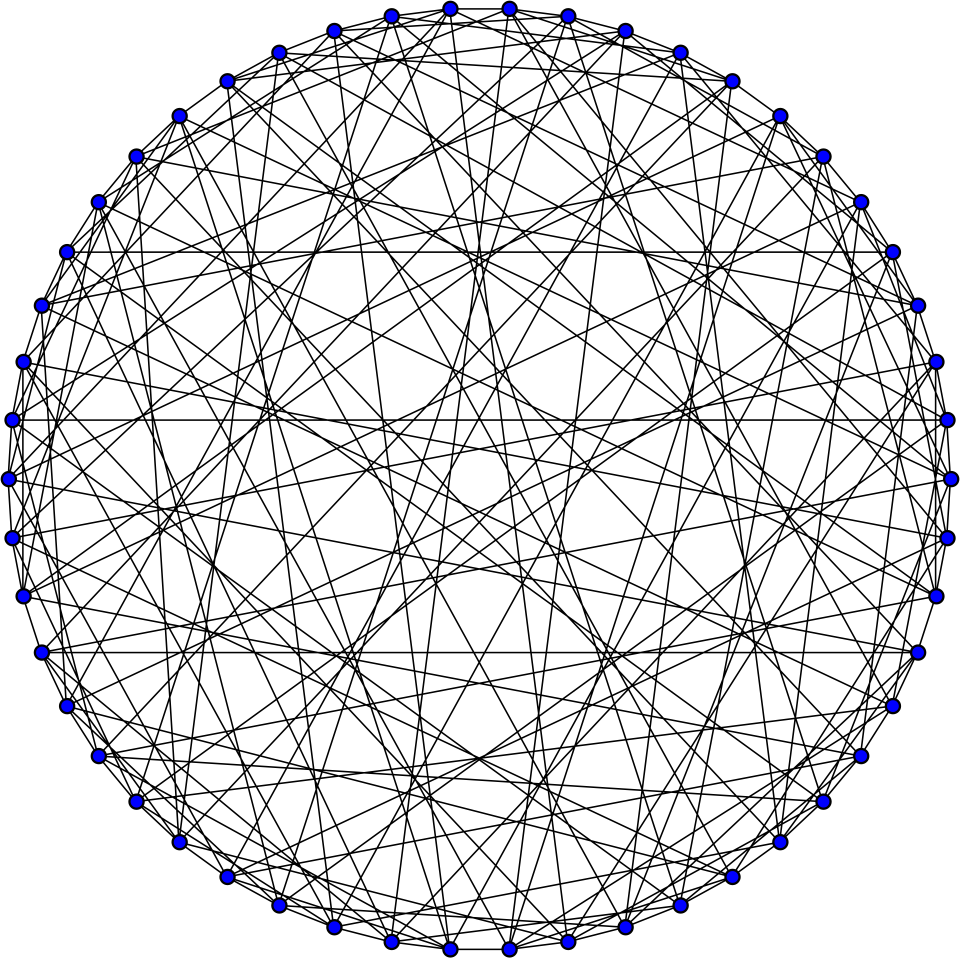
\includegraphics[width=0.5\textwidth]{../../assets/hoffman-singelton-graph.png}
    \caption{Hoffman-Singletonov graf}
    \label{fig:hs_graph}
\end{figure}
\end{frame}

\begin{frame}
\frametitle{Graf valence 57}
\begin{trditev}
    Mooreov graf premera $2$ in stopnje $\Delta = 57$ stoji na $\Delta^2 + 1 = 3250$
    vozliščih. Njegove lastne vrednosti so $57, 7$ in $-8$ z večkratnostmi
    $1, 1729$ in $1520$. Preko zgornje meje Haemersa izvemo, da je moč njegove 
    neodvisne množice največ $400$. Higman in Aschbacher pokažeta, da tak graf, 
    če obstaja, ni vozliščno tranzitiven.
\end{trditev}
    \begin{definicija}
        Graf $G$ je vozliščno tranzitiven, če za poljubni vozišči $u$ in $v$ obstaja
        avtomorfizem $\sigma \in \operatorname{Aut}(G)$, tako da $\sigma(u)= v$.
    \end{definicija}
\end{frame}

\begin{frame}
    \frametitle{Redkost in razširitve Mooreovih grafov}
    \begin{itemize}
        \item[\textbullet] Spodnja meja za red grafov ožine $g=2D+1$
        ter maksimalne stopnje $\Delta$, razširja zgornjo mejo 
        za Mooreove grafe. 

    \end{itemize}
            \begin{trditev}
            \begin{equation*}
        |V(G)| \ge
        \begin{cases}
        \frac{\Delta(\Delta-1)^{(g-1)/2}-1}{\Delta-2}, & g \text{ liho},\\[1em]
        2\frac{(\Delta-1)^{g/2}-1}{\Delta-2}, & g \text{ sodo}.
        \end{cases}
    \end{equation*}
        \end{trditev}
\end{frame}


\begin{frame}
\frametitle{Posplošeni večkotniki}
\begin{definicija}
    Posplošeni $n$-kotnik je geometrija ranga 2 \(\Gamma=(\PP, \LL, \II)\), kjer imamo
točke $\PP$ in premice $\LL$, ki so med seboj povezane z neko relacijo, 
tako, da cela struktura nima podgeometrijskih struktur, ki bi bile običajni manjši
kotniki, ter da se vsaka dva elementa nahajata v nekem običajnem $n$-kotniku.
\end{definicija}

\begin{definicija}
    Pravimo, da je posplošen $n$-kotnik simetričen, oziroma, da je reda $(s, s)$, če je vsaka
premica incidentna s $s + 1$ točkami, in vsaka točka incidentna s $s + 1$ premicami.

V splošnem so posplošeni $n$-kotniki reda $(s, t)$.
\end{definicija}
\end{frame}

\begin{frame}
    \frametitle{Geometrija in posplošeni večkotniki} 
    \begin{trditev}
        Naj bo $\Gamma$ posplošeni $(n \geq 3)$-kotnik reda $(s, s)$, potem velja:
         $|\PP| = |\LL| = \frac{s^n - 1}{s - 1} = s^{n-1} + \ldots + s + 1$.
        Splošneje pa (za red $(s, t)$) velja, da je 
        $|\PP| = (s+1)\frac{(st)^{n/2} - 1}{st - 1}$, $\LL = (t+1)\frac{(st)^{n/2} - 1}{st - 1}$, če $n$ sod,
        in $|\PP| = |\LL| = \frac{s^n - 1}{s - 1}$, če $n$ lih.
    \end{trditev}
\end{frame}

\begin{frame}
    \frametitle{Primer posplošenega večkotnika}
    \begin{definicija}
        Običajni $n$-kotnik je geometrija ranga 2, katere incidenčni graf je cikel 
        dolžine $2n$.
    \end{definicija}
    \begin{zgled}
        Običajni $n$-kotnik je posplošeni natanko $n$-kotnik reda $(1, 1)$. Posledično
        je $2n$-kotnik posplošen Mooreov graf.
    \end{zgled}
\end{frame}

\begin{frame}
    \frametitle{Geometrija in posplošeni večkotniki} 
    \begin{trditev}
    Posplošeni $n$-kotniki reda $(s, t)$, kjer $s\geq2 \lor t\geq2$, obstajajo le za 
    $n \in \{2, 3, 4, 6, 8, 12\}$.
    \end{trditev}
    \begin{zgled}
        V primeru $n=2$ imamo posplošeni 2-kotnik, katerega incidenčni graf je pravzaprav kompletni 
        bipartitni graf $K_{s+1, t+1}$, ki je torej posplošeno Mooreov graf.
    \end{zgled}
\end{frame}

\begin{frame}
    \frametitle{Projektivne ravnine}
    \begin{trditev}
        Definicija projektivne ravnine sovpada z definicijo posplošenega $3$-kotnika, čim je red
        večji od $(1,1)$.
    \end{trditev}
    \begin{definicija}
        Projektivna ravnina je geometrija drugega ranga ($\PP, \LL, \II$), sestavljena iz 
        množice točk $\PP$, množice premic $\LL$ in incidenčne relacije $\II \subset \PP \cup \LL$,
        ki zadoča naslednjim aksiomom:
        \begin{itemize}
            \item[\textbullet] Poljubni dve različni točki ležita na natanko eni premici.
            \item[\textbullet] Poljubni dve različni premici se sekata v natanko eni točki.
            \item[\textbullet] Obstaja vsaj štiri točke, od katerih nobene tri niso kolinearne.
        \end{itemize}
    \end{definicija}
\end{frame}

\begin{frame}
    \frametitle{Projektivne ravnine}
    \begin{izrek}
        Če je projektivna ravnina končna, potem obstaja število $s$, da vsaka premica vsebuje $s+1$ točk,
        in vsaka premica vsebuje $s+1$ točk. Poleg tega, če je $s \equiv 1$ ali $2 \pmod{4}$, 
        potem je brezkvadratni del števila $s$ vsota dveh kvadratov.
    \end{izrek}
    \begin{trditev}
        Klasična oziroma Desarguesova projektivna ravnina $\PG(2, \mathbb{K})$ nad poljem $\mathbb{K}$
        je izpeljana iz vektorskega prostora $V = \mathbb{K}^3$, kjer so točke 
        $\PP = \{\langle \mathbf{x} \rangle \mid \mathbf{x} \in V \setminus \{0\}\}$,
        premice pa $\LL = \{\langle \mathbf{y} \rangle \mid \mathbf{y} \in V \setminus \{0\}\}$,
        kjer je $\langle \mathbf{x} \rangle$ množica vseh neničelnih vektorjev, 
        ki so linearne kombinacije vektorja $\mathbf{x}$,
    \end{trditev}
\end{frame}

\begin{frame}
    \frametitle{Projektivna ravnina}
    \begin{zgled}
        Tako lahko recimo za polje vzamemo končno polje $\mathbb{F}_2 = \{0, 1\}$,
        dobimo $V\setminus \{0\} = \mathbb{F}_2^3 \setminus \{0\} = \{T_{ijk}\mid i,j,k\in\mathbb{F}_2\}$
        in relacijo
        \begin{align*}
T_{100} &\sim {T_{010}, T_{001}, T_{011}} \\
T_{010} &\sim {T_{100}, T_{001}, T_{101}} \\
T_{001} &\sim {T_{100}, T_{010}, T_{110}} \\
T_{110} &\sim {T_{001}, T_{111}, T_{110}} \\
T_{011} &\sim {T_{100}, T_{111}, T_{011}} \\
T_{101} &\sim {T_{010}, T_{111}, T_{101}} \\
T_{111} &\sim {T_{110}, T_{011}, T_{101}}
\end{align*}
    \end{zgled}
\end{frame}

\begin{frame}
\frametitle{Projektivna ravnina}    
\begin{figure}[h]
    \centering
    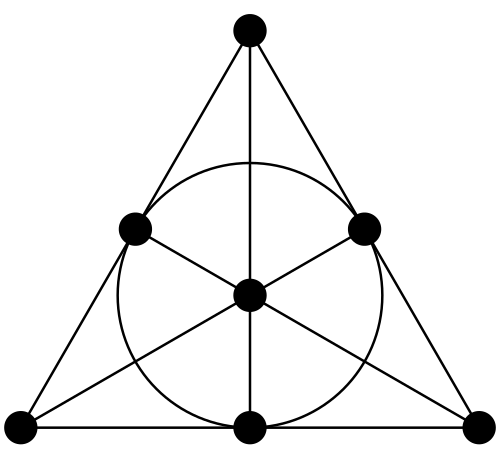
\includegraphics[width=0.3\textwidth]{../../assets/fano-plane.png}%
    \caption{Fanova ravnina (reda $(2,2)$)}
\end{figure}
\end{frame}

\begin{frame}
    \frametitle{Projektivna ravnina}
        \begin{figure}[h]
    \centering
    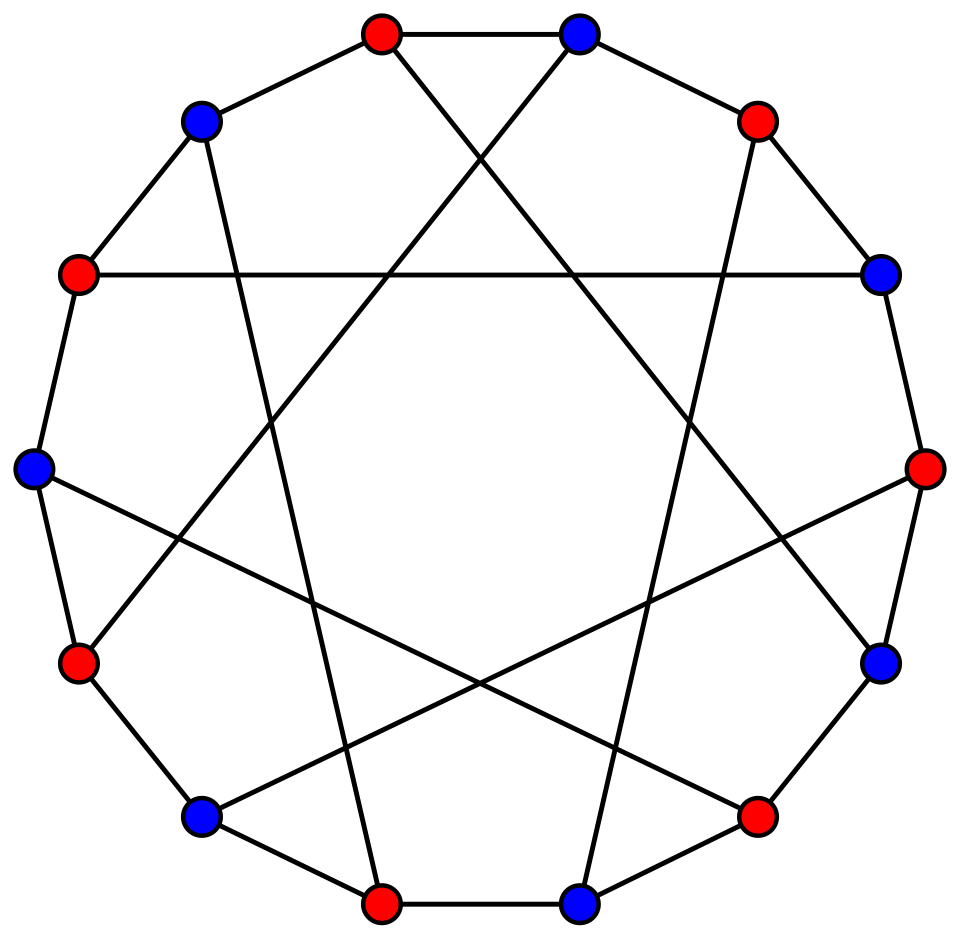
\includegraphics[width=0.3\textwidth]{../../assets/fano-plane-incidence-graph.png}%
    \caption{Incidenčni graf Fanove ravnine}
\end{figure}
\end{frame}

\begin{frame}
    \frametitle{Posplošeni štirikotniki}
    \begin{trditev}
        Šibki posplošeni štirikotnik je geometrija $\Gamma = (\PP, \LL, \II)$, za katero velja:
        \begin{itemize}
            \item [\textbullet] Za vsak nepovezan par $p, L$ obstaja natanko en par $p', L'$, 
            tako, da $p \II L'$ in $p' \II L$.
            \item Vsaka točka leži na vsaj dveh premicah, a ne vseh, in dualno, vsaka premica nosi
            vsaj dve, a ne vse, točke.
        \end{itemize}
    \end{trditev}
        Primer:
        Naj bo $S_6$ simetrična grupa, naj bo $\PP$ množica vseh $15$ transpozicij v $S_6$, $\LL$ 
        množica vseh $15$ involucij brez fiksnih točk. Incidenčna relacija
        naj bo definirana s $\sigma \II \tau \equiv \sigma \tau = \tau \sigma$. 
            Ta geometrija je posplošeni štirikotnik reda $(2, 2)$, oziroma $\operatorname{GQ}(2, 2)$.
\end{frame}


\begin{frame}
    \frametitle{Primer posplošenega štirikotnika}
    \begin{figure}[h]
    \centering
    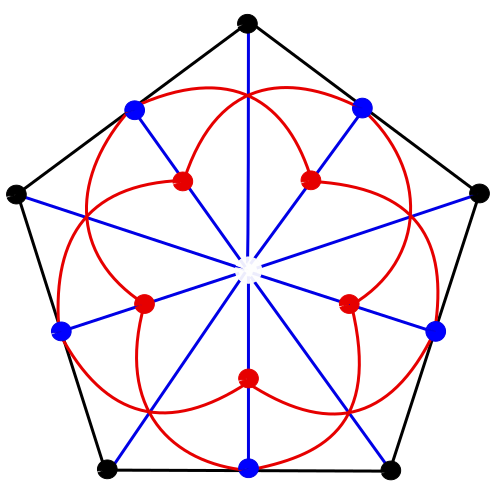
\includegraphics[width=0.3\textwidth]{../../assets/generalized-quadrangle.png}
    \caption{Posplošeni 4-kotnik reda $(2,2)$}
\end{figure}
\end{frame}

\begin{frame}
    \frametitle{Primer posplošenega štirikotnika}
    \begin{figure}[h]
    \centering
    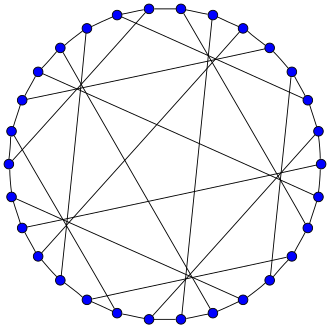
\includegraphics[width=0.3\textwidth]{../../assets/generalized-guadrangle-incidence-graph.png}
    \caption{Incidenčni graf posplošenega 4-kotnika reda $(2,2)$}
\end{figure}
\end{frame}







\begin{frame}
    \frametitle{Posplošeni šestkotniki}
    \begin{figure}[h]
    \centering
    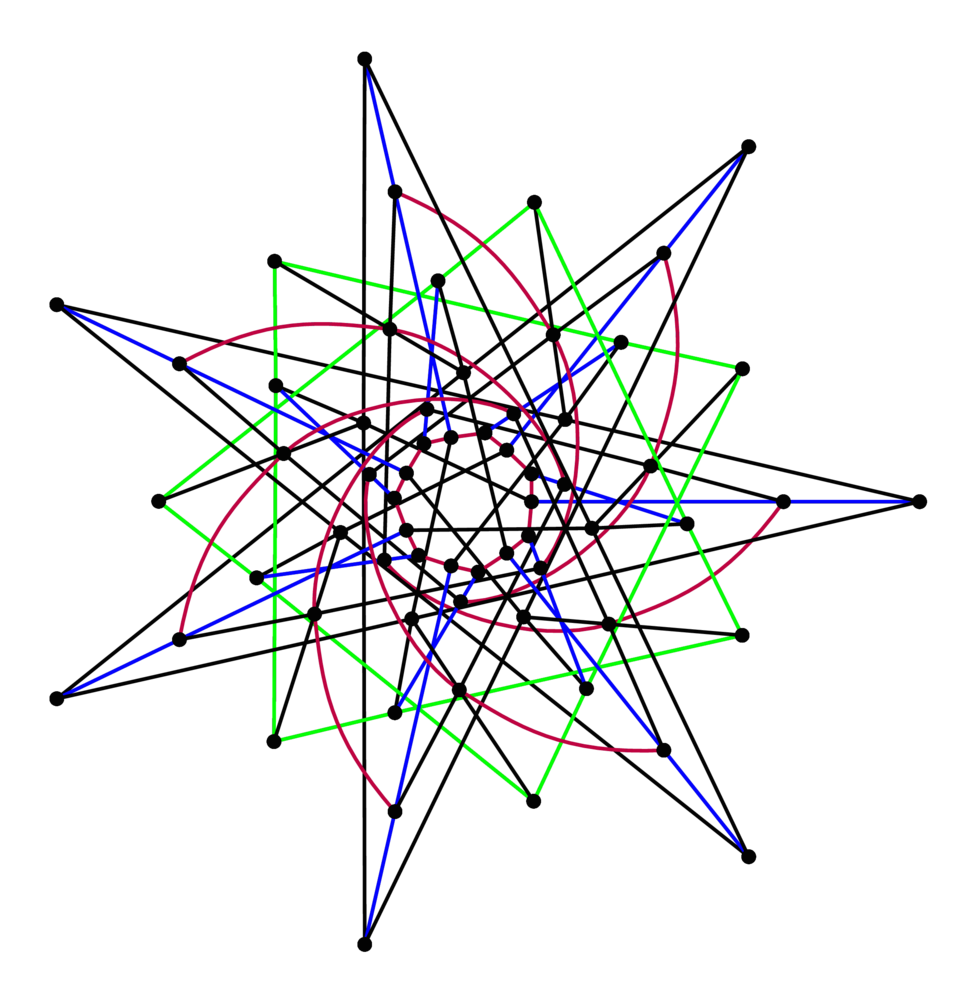
\includegraphics[width=0.5\textwidth]{../../assets/SplitCayleyHexagon.png}
    \caption{Split Cayleyjev šestkotnik reda $(2, 2)$}
    \label{fig:sch_graph}
\end{figure}
\end{frame}

\begin{frame}
    \frametitle{Posplošeni osem in dvanajstkotniki}
    \begin{trditev}
        Incidenčni graf posplošenega osemkotnika ne more biti posplošeno Mooreov, saj mora biti, po Feit-Higmanov izreku,
        $2ss$ kvadrat, kar ni mogoče.
    \end{trditev}
%    \begin{trditev}
%        Posplošeni dvanajstkotnik reda $(1, 1)$ pa je običajen dvanajstkotnik, torej je njegov incidenčni 
%        graf Mooreov, in sicer $C_{24}$.
%    \end{trditev}
\end{frame}

\end{document}
